%Dạng 1
\setcounter{ex}{0}
\section{Điểm biểu diễn số phức}
\subsection{Kiến thức cần nhớ}
\begin{khung}
\subsubsection{Biểu diễn hình học của số phức}
\immini
{
	Biểu diễn hình học của số phức $z=a+bi$ $\left(a,b\in\mathbb{R}\right)$.
	\begin{enumEX}{1}
	\item $M(a;b)$ là điểm biểu diễn của $z$.
	\item $OM=r=\sqrt{a^2+b^2}$ là mô-đun của $z$.
	\end{enumEX}
}
{
	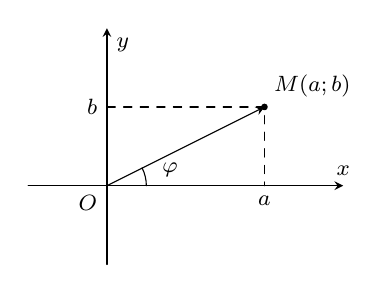
\begin{tikzpicture}[scale=1, font=\footnotesize, line join=round, line cap=round, >=stealth]
	\draw[->] (-1,0)--(3,0)node[above]{$x$};
	\draw[->] (0,-1)--(0,2)node[below right]{$y$};
	\path (0,0)node[below left]{$O$};
	\path (0,1)node[left]{$b$};
	\path (2,0)node[below]{$a$};
	\path (0.8,0.2)node{$\varphi$};
	\draw[fill=black] (2,1)node[above right]{$M(a;b)$} circle(1pt);
	\draw[->] (0,0)--(2,1);
	\draw[dashed] (0,1)--(2,1)--(2,0);
	\draw (0.5,0) arc (0:27:0.5);
	\end{tikzpicture}
}
\end{khung}
\subsection{Bài tập mẫu}
\Opensolutionfile{ans}[ans/ANS-DANG-1]
\begin{khung}
\begin{vd}%[2D4Y1-2]
	Trên mặt phẳng tọa độ, điểm biểu diễn số phức $z=7-6i$ có tọa độ là
	\choice
	{$(-6;7)$}
	{$(6;7)$}
	{$(7;6)$}
	{\True $(7;-6)$}
	\loigiai{
	Điểm biểu diễn số phức $z=7-6i$ có tọa độ là $(7;-6)$.
	}
\end{vd}
\end{khung}
\subsection{Bài tập tương tự và phát triển}

%%==========Câu 1
\begin{ex}%[2D4Y1-2]
\immini{Số phức nào dưới đây có điểm biểu diễn trên mặt phẳng tọa độ là điểm $M$ như hình vẽ bên?
	\choice
	{\True $1-2i$}
	{$i+2$}
	{$i-2$}
	{$1+2i$}
}{\begin{tikzpicture}[scale=1,>=stealth]
	\draw[->] (-1,0)--(2,0)node[below right]{$x$};
	\draw[->] (0,-2.5)--(0,1)node[left]{$y$};
	\fill (0,0)node[below left]{$O$} (1,-2)circle(1.5pt);
	\draw[dashed] (1,0)node[above]{$1$}--(1,-2)node[below right]{$M$}--(0,-2)node[left]{$-2$};
\end{tikzpicture}}
	\loigiai{
	Vì $M(1;-2)\Rightarrow$ $M$ là điểm biểu diễn của số phức $z=1-2i$.}
\end{ex}

%%==========Câu 2
\begin{ex}%[2D4Y1-2]
	\immini{Điểm $M$ trong hình bên là điểm biểu diễn của số phức $z$. Mệnh đề nào sau đây đúng?
	\choice{\True Số phức $z$ có phần thực là $3$ và phần ảo là $-4$}
	{Số phức $z$ có phần thực là $3$ và phần ảo là $-4i$}
	{Số phức $z$ có phần thực là $-4$ và phần ảo là $3$}
	{Số phức $z$ có phần thực là $-4$ và phần ảo là $3i$}
	}{
	\begin{tikzpicture}[line cap=round, line join=round,font=\footnotesize,>=stealth, scale=.6]
	\tikzset{label style/.style={font=\footnotesize}}
	\draw[->] (-1,0)--(0,0)node[below left]{$O$}--(4,0)node[above]{$x$};
	\draw[->] (0,-5)--(0,1)node[left]{$y$};
	\draw[dashed] (0,-4)node[left]{$-4$}--(3,-4)node[below right]{$M$}--(3,0)node[above]{$3$};
	\draw[fill=black] (3,0) circle (1pt)
	(0,-4) circle (1pt)
	(3,-4) circle (1pt)
	(0,0) circle (1pt);
	\end{tikzpicture}
	}
	\loigiai{
	Số phức $z$ có phần thực là $3$ và phần ảo là $-4$.
	}
\end{ex}

%%==========Câu 3
\begin{ex}%[2D4Y1-2]
	\immini{
	Điểm nào trong hình vẽ bên là điểm biểu diễn số phức \break $z=-1+2i$?
	\choice
	{$N$}	
	{$P$}
	{$M$}
	{\True $Q$}
	}
	{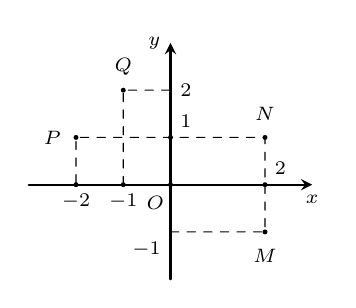
\begin{tikzpicture}[scale=0.6,font=\large,line join=round,line cap=round,>=stealth]
	\path 
	(0,0) coordinate (O)
	(2,-1) coordinate (M) (2,1) coordinate (N) (-2,1) coordinate (P) (-1,2) coordinate (Q)
	(-1,0) coordinate (A)node[below ]{\scriptsize $ -1 $}
	(2,0) coordinate (B)node[above right]{\scriptsize $ 2 $}
	(-2,0) coordinate (C)node[below ]{\scriptsize $ -2 $}
	(0,1) coordinate (D)node[above right]{\scriptsize $ 1 $}
	(0,2) coordinate (E)node[right]{\scriptsize $ 2 $}
	(0,-1) coordinate (F)node[below left]{\scriptsize $ -1 $}
	;
	\draw[thick,->] (-3,0)--(0,0)--(3,0) node[below]{\scriptsize $x$};
	\draw[thick,->] (0,-2) --(0,3) node[left]{\scriptsize $y$};
	\draw[dashed] (0,-1)--(M)--(N)--(P)--(-2,0) (-1,0)--(Q)--(0,2);
	\foreach \p/\r in {M/-90,N/90,P/180,Q/90,O/230}
	\fill (\p) circle (1.5pt) node[shift={(\r:3mm)}]{\scriptsize $\p$};
	\foreach \p in {A,B,C,D}
	\fill (\p) circle (1.5pt) ;
	\end{tikzpicture}
	}
	\loigiai{
	Điểm biểu diễn số phức $z=-1+2i$ là $Q(-1;2)$.	
	}
\end{ex}

%%==========Câu 4
\begin{ex}%[2D4Y1-2]
	\immini{
	Số phức nào dưới đây có điểm biểu diễn trên mặt phẳng tọa độ là điểm $M$ như hình vẽ bên?
	\choice
	{$z_4=2+i$}	
	{$z_2=1-2i$}
	{\True $z_3=-2+i$}
	{$z_1=1-2i$}
	}{\begin{tikzpicture}[scale=0.8,line join=round,line cap=round,>=stealth]
	\draw[->] (-3,0)--(1,0) node[below]{\scriptsize $x$};
	\draw[->] (0,-1) --(0,2) node[left]{\scriptsize $y$};
	\draw[dashed] (-2,0)node[below]{$-2$}--(-2,1)node[above]{$M$}--(0,1)node[right]{$1$};
	\fill (-2,1) circle (1.5pt) ;
	\end{tikzpicture}
	}
	\loigiai{
	Điểm $M(-2;1)$ biểu diễn số phức $z_3=-2+i$. 
	}
\end{ex}

%%==========Câu 5
\begin{ex}%[2D4B1-2]
	\immini{
	Cho số phức $z= (1+i)(2-i)$. Điểm nào trong hình vẽ dưới đây là điểm biểu diễn của $z$?
	\choice
	{$M$}
	{$P$}
	{$N$}
	{\True $Q$}
	}{
	\begin{tikzpicture}[>=stealth,line join=round,line cap=round,font=\footnotesize,scale=0.6]
	\draw[->] (-3.5,0)--(3.5,0) node[below]{\scriptsize $x$};
	\draw[->] (0,-1.5)--(0,3.5) node[left]{\scriptsize $y$};
	\fill[name=O] (0,0) circle (1.2pt) node[below left] {\scriptsize $O$}; 
	\coordinate[label=above right:{\scriptsize $M$}] (M) at (1,3);
	\coordinate[label=above left:{\scriptsize $N$}] (N) at (-1,3);
	\coordinate[label=below:{\scriptsize $P$}] (P) at (-3,-1);
	\coordinate[label=above:{\scriptsize $Q$}] (Q) at (3,1);
	\coordinate[label=above:{\scriptsize $-3$}] (-3x) at (-3,0);
	\coordinate[label=below left:{\scriptsize $-1$}] (-1x) at (-1,0);
	\coordinate[label=below:{\scriptsize $1$}] (1x) at (1,0);
	\coordinate[label=below:{\scriptsize $3$}] (3x) at (3,0);
	\coordinate[label=right:{\scriptsize $-1$}] (-1y) at (0,-1);
	\coordinate[label=left:{\scriptsize $1$}] (1y) at (0,1);
	\coordinate[label=above right:{\scriptsize $3$}] (3y) at (0,3);
	\draw[dashed] (-3x)--(P)--(-1y)
	(-1x)--(N)--(M)--(1x)
	(1y)--(Q)--(3x);
	\foreach \p in {M,N,P,Q,{-3,0},{-1,0},{1,0},{3,0},{0,-1},{0,1},{0,3}}
	\fill (\p) circle (1.2pt);
	\end{tikzpicture}
	}
	\loigiai{
	Ta có $z = (1+i)(2-i)= 3 + i$.\\
	Vậy điểm biểu diễn cho số phức $z$ là $Q(3;1)$.
	}
\end{ex}

%%==========Câu 6
\begin{ex}%[2D4Y1-2]
	Trên mặt phẳng tọa độ, điểm biểu diễn số phức $z=(1+2i)^2$ là điểm nào dưới đây? 
	\choice
	{\True $P(-3;4)$}
	{$Q(5;4)$}
	{$N(4;-3)$}
	{$M(4;5)$}
	\loigiai{ 
	Ta có $z=(1+2i)^2=-3+4i$ có điểm biểu diễn là $P(-3;4)$.
	}
\end{ex}

%%==========Câu 7
\begin{ex}%[2D4Y1-2]
	Biết $M(1;-2)$ là điểm biểu diễn số phức $\overline{z}$, số phức $z$ bằng
	\choice
	{$2+i$}
	{\True $1+2i$}
	{$2-i$}
	{$1-2i$}
	\loigiai{
	Vì $M(1;-2)$ là điểm biểu diễn của số phức $\overline{z}$ nên $\overline{z}=1-2i$. Từ đó suy ra $z=1+2i$.
	}
\end{ex}

%%==========Câu 8
\begin{ex}%[2D4Y1-2]
	Gọi $M$ và $M'$ lần lượt là các điểm biểu diễn cho các số phức $z$ và $\overline{z}$. Xác định mệnh đề đúng.
	\choice
	{\True $M$ và $M'$ đối xứng với nhau qua trục hoành}
	{$M$ và $M'$ đối xứng với nhau qua trục tung}
	{$M$ và $M'$ đối xứng với nhau qua gốc tọa độ}
	{Ba điểm $O, M, M'$ thẳng hàng}
	\loigiai{
	\immini{
	Viết $z=a+bi\Rightarrow \overline{z}=a-bi$, với $a,b\in\mathbb{R}$.\\
	Suy ra các điểm biểu diễn cho các số phức $z$ và $\overline{z}$ lần lượt là $M(a;b)$ và $M'(a;-b)$.\\
	Vậy $M$ và $M'$ đối xứng với nhau qua trục hoành.
	}
	{
	\begin{tikzpicture}[scale=0.7, font=\footnotesize, line join=round, line cap=round, >=stealth]
	\\coordinate (O) at (0,0);
	\draw[->](-1,0)--(3,0)node[below]{$x$};
	\draw[->](0,-1.5)--(0,1.5)node[right]{$y$};
	\clip(-1,-1.5) rectangle (3,1.5);
	\coordinate (M) at (2,1);
	\coordinate (M') at (2,-1);
	\draw[dashed](0,1)node[left]{$b$}--(M)--(2,0)node[below right]{$a$}--(M')--(0,-1)node[left]{$-b$};
	\foreach \t/\g in {M/0,M'/0,O/-45}{
		\fill (\t) circle (1pt) node[shift={(\g:7pt)},font=\scriptsize]{$ \t $};
	}
	\end{tikzpicture}
	}
	}
\end{ex}

%%==========Câu 9
\begin{ex}%[2D4Y1-2]
\immini{Trong hình vẽ bên, điểm $P$ biển diễn số phức $z_1$, điểm $Q$ biểu diễn số phức $z_2$. Tìm số phức $z=z_1+z_2$?
	\choice
	{\True $1+3i$}
	{$-3+i$}
	{$-1+2i$}
	{$2+i$}}{
	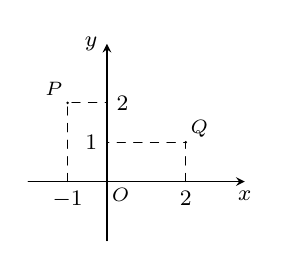
\begin{tikzpicture}[scale=.5, font=\footnotesize, line join=round, line cap=round, >=stealth]
	\draw[->] (-2,0)--(3.5,0) node [below]{$x$};
	\draw[->] (0,-1.5)--(0,3.5) node [left]{$y$};
	\clip (-2,-1.5) rectangle (3.5,3.5);
	\path (-1,2) coordinate (P)
	(2,1) coordinate (Q)
	(0,0) coordinate (O);
	\draw[dashed] (-1,0)--(-1,2)--(0,2) (2,0)--(2,1)--(0,1);
	\draw (-1,0) node[below] {$-1$};
	\draw (2,0) node[below] {$2$};
	\draw (0,1) node[left] {$1$};
	\draw (0,2) node[right] {$2$};
	\foreach \t/\g in {P/135,Q/45,O/-45}{
		\fill (\t) circle (1pt) node[shift={(\g:7pt)},font=\scriptsize]{$ \t $};
	}
	\end{tikzpicture}}
	\loigiai{Nhìn vào hình vẽ trên ta thấy $z_1=-1+2i$, $z_2=2+i$.\\
	Khi đó $z_1+z_2=1+3i$.	
	}
\end{ex}

%%==========Câu 10
\begin{ex}%[2D4B1-2]
	Cho số phức $z = 1 + \sqrt{3}i$. Nghịch đảo của $z$ có điểm biểu diễn là
	\choice
	{$N\left(\dfrac{1}{2};\dfrac{\sqrt{3}}{2}\right)$}
	{$M\left(\dfrac{1}{2};-\dfrac{\sqrt{3}}{2}\right)$}
	{$P\left(\dfrac{1}{4};\dfrac{\sqrt{3}}{4}\right)$}
	{\True $Q\left(\dfrac{1}{4};-\dfrac{\sqrt{3}}{4}\right)$}
	\loigiai{
	Ta có $\dfrac{1}{z}=\dfrac{1}{1+\sqrt{3}i}=\dfrac{1-\sqrt{3}i}{4}=\dfrac{1}{4} - \dfrac{\sqrt{3}}{4}i$.\\
	Vậy điểm biểu diễn cho số phức $\dfrac{1}{z}$ là điểm $Q\left(\dfrac{1}{4};-\dfrac{\sqrt{3}}{4}\right)$.
	}
\end{ex}

%%==========Câu 11
\begin{ex}%[2D4Y1-2]
	Cho số phức $z_1 = 1-2i$, $z_2 = -3+i$. Điểm nào dưới đây là điểm biểu diễn của số phức $w= z_1+z_2$ trên mặt phẳng tọa độ?
	\choice
	{$N(4;-3)$}
	{$M(2;-5)$}
	{\True $P(-2;-1)$}
	{$Q(-1;7)$}
	\loigiai{
	Ta có $w = z_1 + z_2 = (1-2i) + (-3 +i)= -2 -i$.\\
	Vậy điểm biểu diễn cho số phức $w$ là $P(-2;-1)$.
	}
\end{ex}

%%==========Câu 12
\begin{ex}%[2D4Y1-2]
	Cho số phức $z = 1-2i$. Điểm nào dưới đây là điểm biểu diễn của số phức $w=iz$ trên mặt phẳng tọa độ?
	\choice
	{$Q(1;2)$}
	{\True $N(2;1)$}
	{$M(1;-2)$}
	{$P(-2;1)$}
	\loigiai{
	Ta có $w=iz = i(1-2i)= 2 + i$.\\
	Vậy điểm biểu diễn cho số phức $w$ là $N(2;1)$.
	}
\end{ex}

%%==========Câu 13
\begin{ex}%[2D4B1-2]
	Cho số phức $z = 3-2i$. Khi đó số phức $w = z +i\overline{z}$ có điểm biểu diễn trên mặt phẳng tọa độ là điểm nào dưới đây?
	\choice
	{$H(1;-5)$}
	{$G(5;-5)$}
	{\True $E(1;1)$}
	{$F(5;1)$}
	\loigiai{
	Ta có $w= z + i\overline{z}= (3 -2i)+ i(3+2i)=3-2i + 3i -2= 1+i$.\\
	Vậy điểm biểu diễn cho số phức $w$ là $E(1;1)$.
	}
\end{ex}

%%==========Câu 14
\begin{ex}%[2D4B1-2]
	Cho số phức $z$ thỏa mãn $iz + 2-i=0$. Khoảng cách từ điểm biểu diễn của $z$ trên mặt phẳng tọa độ $Oxy$ đến điểm $M(3;-4)$ bằng
	\choice
	{$2\sqrt{5}$}
	{$\sqrt{13}$}
	{\True $2\sqrt{10}$}
	{$2\sqrt{2}$}
	\loigiai{
	Ta có $iz + 2-i=0\Leftrightarrow z =\dfrac{-2+i}{i}=1+2i$.\\
	Khi đó điểm biểu diễn cho $z$ là $A(1;2)\Rightarrow \overrightarrow{MA}=(-2;6)$.\\
	Vậy khoảng cách từ $A$ đến $M$ là $|\overrightarrow{MA}|=\sqrt{(-2)^2 + 6^2}=2\sqrt{10}$.
	}
\end{ex}

%%==========Câu 15
\begin{ex}%[2D4B1-2]
	Trên mặt phẳng phức, cho điểm $A$ biểu diễn số phức $3-2i$, điểm $B$ biểu diễn số phức $-1 + 6i$. Gọi $M$ là trung điểm của $AB$. Khi đó điểm $M$ biểu diễn số phức nào trong các số phức sau?
	\choice
	{$1-2i$}
	{$2-4i$}
	{$2+4i$}
	{\True $1+2i$}
	\loigiai{
	Ta có $A(3;-2)$ và $B(-1;6)$.\\
	Vì $M$ là trung điểm $AB$ nên $\heva{&x_M=\dfrac{3+(-1)}{2}=1\\&y_M=\dfrac{-2+6}{2}=2}\Rightarrow M(1;2)$.\\
	Vậy điểm $M$ biểu diễn cho số phức $1+2i$.
	}
\end{ex}

%%==========Câu 16
\begin{ex}%[2D4B1-2]
	Trên mặt phẳng phức, các điểm $A$, $B$, $C$ lần lượt là các điểm biểu diễn của các số phức $z_1 = -3i$ và $z_2 = 2-2i$, $z_3=-i-5$. Số phức $z$ biểu diễn trọng tâm $G$ của tam giác $ABC$ là
	\choice
	{\True $z = -1 -2i$}
	{$z = -2 +i$}
	{$z = -1 -i$}
	{$z = -1 +i$}
	\loigiai{
	Ta có $A(0;-3)$, $B(2;-2)$, $C(-5;-1)$.\\
	Vì $G$ là trọng tâm $\triangle ABC$ nên $\heva{&x_G=\dfrac{0+2+(-5)}{3}=-1\\&y_G=\dfrac{-3+(-2)+(-1)}{3}=-2}\Rightarrow G(-1;-2)$.\\
	Vậy điểm $G$ biểu diễn cho số phức $z= -1-2i$.
	}
\end{ex}

%%==========Câu 17
\begin{ex}%[2D4B1-2]
	Nếu điểm $M(x;y)$ là điểm biểu diễn hình học của số phức $z$ trong mặt phẳng tọa độ $Oxy$ thoả mãn $OM=4$ thì
	\choice
	{$|z|=\dfrac{1}{4}$}
	{\True $|z|=4$}
	{$|z|=16$}
	{$|z|=2$}
	\loigiai{Theo bài ra $OM=4\Rightarrow\sqrt{x^2+y^2}=4\Rightarrow|z|=4$.}
\end{ex}

%%==========Câu 18
\begin{ex}%[2D4B1-2]
	Cho các số phức $z$, $z'$ có biểu diễn hình học lần lượt là các điểm $M$, $M'$ trong mặt phẳng tọa độ $Oxy$. Nếu $OM=2OM'$ thì
	\choice
	{\True $|z|=2|z'|$}
	{$z'=2z$}
	{$z=2z'$}
	{$|z'|=2|z|$}
	\loigiai{
	Ta có $|z|=OM$, $|z'|=OM'$. Do đó, nếu $OM=2OM'$ thì $|z|=2|z'|$.
	}
\end{ex}

%%==========Câu 19
\begin{ex}%[2D4B1-2]
	Gọi $ M, N, P $ lần lượt là các điểm biểu diễn của các số phức $ z_1=1+i $, $ z_2=8+i $, $ z_3=1-3i $ trong mặt phẳng phức $ Oxy $. Khẳng định nào sau đây là khẳng định đúng?
	\choice
	{\True $ \triangle MNP $ vuông}
	{$ \triangle MNP $ đều}
	{$ \triangle MNP $ cân}
	{$ \triangle MNP $ vuông cân}
	\loigiai{
	Ta có $ M(1; 1), N(8; 1), P(1; -3) $.\\
	Dễ dàng tính được $ MN=7, NP=\sqrt{65}, MP=4 \Rightarrow MN^2+MP^2=NP^2 $.\\
	Vậy tam giác $ MNP $ vuông tại $ M $.
	}
\end{ex}

%%==========Câu 20
\begin{ex}%[2D4B1-2]
	\immini{
	Cho tam giác $ABC$ như hình vẽ. Biết trọng tâm $G$ của tam giác $ABC$ là điểm biểu diễn của số phức $z$. Tìm phần ảo của số phức $\overline{z}$.
	\choice
	{$1$}
	{\True $-1$}
	{$-i$}
	{$i$}
	}{
	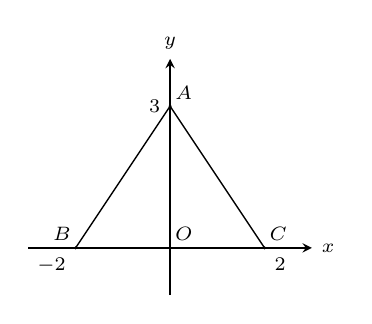
\begin{tikzpicture}[line width=0.5pt,>=stealth,x=1cm,y=1cm,scale=0.6,font=\scriptsize] 
	\path (0,0) coordinate (O)
	(0,3) coordinate (A)
	(-2,0) coordinate (B)
	(2,0) coordinate (C);
	\draw[->] (-3,0) -- (3,0) node[right] {$x$};
	\draw[->] (0,-1) -- (0,4) node[above] {$y$};
	\draw (-2,0) node[below left]{$-2$};
	\draw (2,0) node[below right]{$2$};
	\draw (0,3) node[left]{$3$};
	\draw (A)--(B)--(C)--cycle;
	\foreach \t/\g in {O/45,A/45,B/135,C/45}{
		\fill (\t) circle (1pt) node[shift={(\g:7pt)},font=\scriptsize]{$ \t $};
	}
	\end{tikzpicture}
	}
	\loigiai{
	Theo giả thiết, ta có $A(0;3)$, $B(-2;0)$, $C(2;0)$.\\
	Tọa độ trọng tâm $G$ của tam giác $ABC$ là $G\left( 0;1\right)$ nên $z=i \Rightarrow\overline{z}=-i.$ 
	}
\end{ex}
\Closesolutionfile{ans}
\subsection{Bảng đáp án}
\inputansbox{10}{ans/ANS-DANG-1}